\documentclass[UTF8]{ctexart}
\usepackage{graphicx}
\usepackage{subfigure}
\usepackage{amsmath}
\usepackage{geometry}
\usepackage{enumerate}
\usepackage{cite}
\usepackage{booktabs}
\usepackage{listings}
\usepackage{titletoc}

\lstset{language=C++}
\lstset{breaklines}%这条命令可以让LaTeX自动将长的代码行换行排版
\lstset{extendedchars=false}%这一条命令可以解决代码跨页时,章节标题,页眉等汉字不显示的问题

\geometry{left=2cm,right=2cm,top=2cm,bottom=2cm}

\title{\heiti 《计算空气动力学》 \\ 大作业}
\author{SX1501021 仓宇}
\date{\today}

\bibliographystyle{plain}

\begin{document}
\maketitle
\setcounter{page}{0}
\thispagestyle{empty}
\clearpage

\tableofcontents
\clearpage

\section{问题描述}
求解无粘条件下NACA0012翼型的2维平面流场。流场网格是由三角形单元组成的非结构网格,使用有限体积方法求解流场的2维Euler方程。网格文件为data文件夹下的naca0012.grd文件。全流场的网格如下左图所示,右图是翼型周围的网格:
\begin{figure}[htbp]
\centering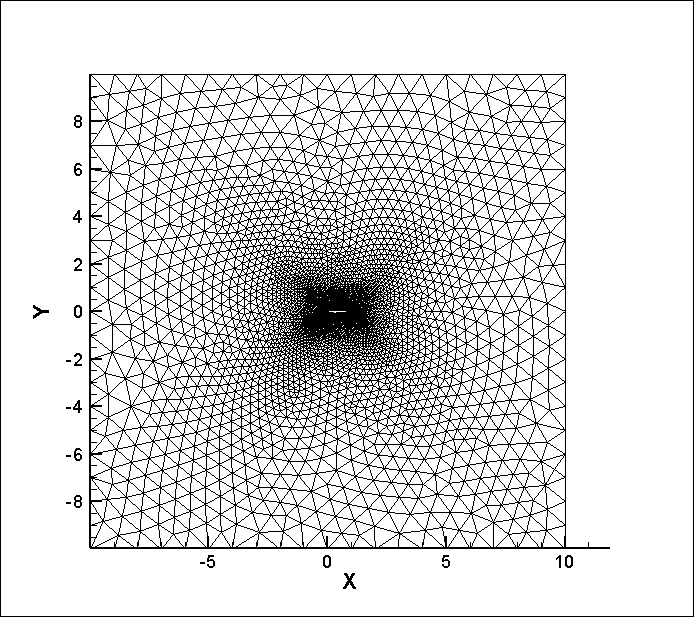
\includegraphics[width=5.5cm,height=4.5cm]{../data/mesh_naca0012.png}
\centering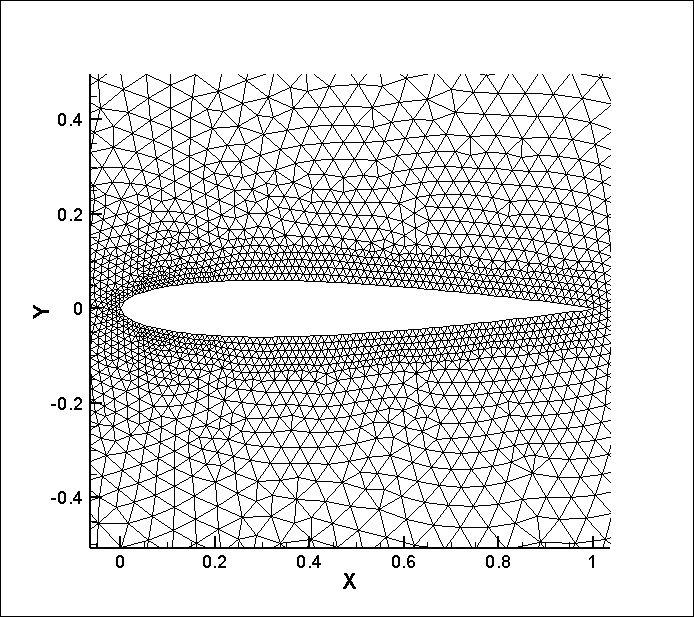
\includegraphics[width=5.5cm,height=4.5cm]{../data/mesh_naca0012_local.png}
\caption{用于NACA0012翼型的非结构网格}
\end{figure}

\section{问题分析}
本文采用Jameson中心格式来求解二维Euler方程。在空间离散上采用的是有限体积法,时间上采用的是四步显式Runge-Kutta迭代求得最后的定常解。人工耗散项为守恒变量的二阶和四阶差分项。边界条件采用的是无反射边界条件,并采用当地时间步长进行加速收敛。

\subsection{基本方程}
由于不考虑粘性,二维NS方程可简化为Euler方程。欧拉方程是质量,动量,能量守恒定理的表达。在边界为S,面积为Ω的二维区域,方程可以写成以下形式:
\begin{equation}
\frac{\partial}{\partial t} \iint_{\Omega} W d\Omega + \int_{S} (Fdy-Gdx) = 0
\end{equation}

\indent 其中,$x,y$是笛卡尔坐标,$W$是守恒量矢量,$F,G$是流动矢量,具体形式如下:
\begin{equation}
W={\begin{bmatrix} \rho \ \rho U \ \rho V \ \rho E \end{bmatrix}}^\mathrm{T}
\end{equation}

\begin{equation}
F={\begin{bmatrix} \rho U \ \rho U^2 + P \ \rho UV \ \rho UH \end{bmatrix}}^\mathrm{T}
\end{equation}

\begin{equation}
G={\begin{bmatrix} \rho V \ \rho UV \ \rho V^2 + P \ \rho VH \end{bmatrix}}^\mathrm{T}
\end{equation}

\indent $\rho,P,H,E$分别是密度,压强,单位质量总焓和单位质量总能量;$U,V$是速度矢量的笛卡尔坐标系下的分量。这些变量之间的关系如下:
\begin{equation}
\rho E=P/(\gamma-1)+\rho (U^2+V^2)/2
\end{equation}

\begin{equation}
\rho H=\rho E + P
\end{equation}

\subsection{空间离散}
计算区域被划分为有限数量的非重叠单元,并且积分形式的守恒方程应用到每个单元。因为考虑到时间,任何单元的体积都可视作常数,

\subsection{人工耗散}

\subsection{时间离散}

\subsection{边界条件}

\section{编程实现}

\subsection{数据存储结构}

\subsection{程序流程}

\section{结果分析}

\subsection{Ma=0.3}

\subsection{Ma=0.8}

\subsection{Ma=1.2}

\section{总结}


\end{document}
